\documentclass[a4paper,fleqn]{cas-dc}
\usepackage[numbers]{natbib}
\usepackage{amsmath,amssymb,amsthm}
\usepackage{booktabs}
\usepackage{algorithm}
\usepackage{algpseudocode}

\theoremstyle{plain}
\newtheorem{definition}{Definition}
\newtheorem{lemma}{Lemma}
\newtheorem{proposition}{Proposition}
\newtheorem{theorem}{Theorem}
\newtheorem{corollary}{Corollary}
\theoremstyle{remark}
\newtheorem{remark}{Remark}

\newcommand{\sys}{\mbox{QuantGhost}}

\begin{document}

\shorttitle{QuantGhost: deployment-robust weight steganography}
\shortauthors{E.~A.~Winanto et~al.}

\title[mode=title]{Surviving Sanitization with \sys: Deployment-Robust and Stealthy Steganography in Neural-Network Weights}

\author[1,2]{Eko Arip Winanto}[orcid=0000-0003-3274-1885]
\ead{winanto@graduate.utm.my}
\author[1,3]{Mohd Yazid Idris}
\author[4]{Kurniabudi}
\cormark[1]
\ead{kurniabudi@unama.ac.id}

\affiliation[1]{organization={Faculty of Computing, Universiti Teknologi Malaysia},
  city={Johor Bahru}, postcode={81310}, country={Malaysia}}
\affiliation[2]{organization={Department of Computer Engineering, Dinamika Bangsa University}, city={Jambi},postcode={36138}, country={Indonesia}}
\affiliation[3]{organization={MaGIC-X (Media and Games Innovation Centre of Excellence), Universiti Teknologi Malaysia}, city={Johor Bahru}, postcode={81310}, country={Malaysia}}
\affiliation[4]{organization={Master of Information System, Dinamika Bangsa University}, city={Jambi}, postcode={36138}, country={Indonesia}}
\cortext[cor1]{Corresponding author.}

\begin{abstract}
Pre-trained networks now circulate as shared artifacts, so a tampered checkpoint on a
popular hub reaches every downstream user. Prior attacks such as StegoNet, EvilModel
and MaleficNet show that float32 weights can hide megabytes of data at negligible
accuracy cost, yet they assume the model is run exactly as published. It rarely is.
Before reaching an edge or medical (IoMT) device a model is quantized to INT8, pruned
and fine-tuned, and we confirm on real networks that these routine steps erase
mantissa-bit payloads entirely. We then show that they need not. We present \sys, a
quantization-aware embedding that writes each payload bit into the INT8 code that
quantization produces, so it survives by construction; placing every weight at a random point inside its code's bin
keeps the mantissa distribution natural and defeats byte-image steganalysis, while
redundant coding carries the payload through pruning and fine-tuning. On a real
ResNet-50 a $3.2$\,MB payload survives INT8 at $99.9999\%$ fidelity; on a real
ResNet-56 the attack costs $0.19$ percentage points of accuracy; and against the
released Model X-Ray detector on a diverse model population our payload is
indistinguishable from benign weights ($0.50$, chance), whereas the prior attack is
flagged ($0.81$). Underlying these results is a fundamental limit we prove, the
capacity-robustness-stealth trilemma: at most two of the three hold together, and any
permutation-invariant channel, ours or prior watermarking, is bounded by the sum of
$k_h k_w$ over convolution layers. A faithful neuron permutation, function-preserving
to $10^{-14}$, removes the high-capacity payload but leaves that small invariant
channel intact, which suffices to bootstrap recovery. We also propose a sub-quantum
residual detector that flags QuantGhost (ROC-AUC $1.0$) where byte-level steganalysis
fails. Deployment sanitization alone is therefore incomplete, and we set out what closing
the gap requires.
\end{abstract}

\begin{highlights}
\item Naive weight-steganography payloads are fully erased by INT8 quantization on real models.
\item \sys, a quantization-aware distribution-preserving embedding, survives INT8, pruning and fine-tuning, costing $0.19$\,pp accuracy on a real ResNet-56.
\item It evades the released Model X-Ray detector on a diverse model zoo ($0.50$, chance) where prior art is detected ($0.81$).
\item We prove a capacity-robustness-stealth trilemma with a tight $\sum k_h k_w$ bound on the permutation-invariant channel.
\item A faithful neuron permutation on ResNet-18 destroys the high-capacity payload but a $196$-bit invariant channel survives, so sanitization is incomplete.
\end{highlights}

\begin{keywords}
neural network steganography \sep stegomalware \sep model supply chain \sep
quantization \sep steganalysis \sep deep learning security
\end{keywords}

\maketitle

% =====================================================================
\section{Introduction}\label{sec:intro}
Sharing pre-trained models is now the default way to build machine-learning systems.
Practitioners pull a checkpoint from a hub, adapt it, and ship it. That convenience
turns the model file itself into a supply-chain asset, and a tampered file propagates
to everyone who reuses it, the same dynamic that makes poisoned packages and
trojaned binaries dangerous, transplanted into the weight space of a network
\citep{gu2017badnets,liu2018trojaning,digregorio2026insecurity}. The carrier is generous: a float32
weight devotes most of its mantissa to precision the task never needs, and StegoNet
\citep{liu2020stegonet}, EvilModel \citep{wang2021evilmodel,wang2022evilmodel2} and
MaleficNet \citep{hitaj2022maleficnet,hitaj2025trust} exploit exactly that slack to
hide megabytes of payload with accuracy loss below one percent.

These attacks assume a static artefact, a condition the deployment pipeline violates. A
model is almost never deployed bit-for-bit as published. On the way to a phone, a sensor, or a bedside IoMT
monitor it is compressed: post-training INT8 quantization \citep{jacob2018quantization},
magnitude or structured pruning \citep{han2015learning,han2016deepcompression}, and a
round of fine-tuning on local data. We show in Section~\ref{sec:motiv}, on real
networks, not toy ones, that this pipeline annihilates a mantissa-bit payload:
recovery falls to a coin flip at every embedding depth. Worse for the attacker, the
very same transforms have been put forward as defenses, alongside neuron permutation
(NeuPerm), which shuffles channel order using the network's permutation symmetry and
scrambles any position-dependent payload at no accuracy cost
\citep{gilkarov2025neuperm}. Detection has matured in parallel: Model X-Ray casts the
weights to a grayscale image and learns, from a handful of examples, to tell stego
from benign \citep{gilkarov2026modelxray}.

So the question that has not been answered is sharp. \emph{Can a payload survive the
full deployment pipeline and still be stealthy and accuracy-preserving?} We answer it
constructively, but the more durable contribution is what the answer exposes: a
fundamental three-way limit, a \emph{capacity-robustness-stealth trilemma}, that
constrains every weight-embedding scheme, ours and prior watermarking alike. We develop
the work in three movements.

First, the attack, which we name \sys. Rather than hiding in the mantissa, it writes
each payload bit into the INT8 code that quantization will produce, so re-quantization
recovers it exactly (Section~\ref{sec:method}). Stealth follows from two design choices:
the payload is encrypted, and each weight is placed at a random point \emph{inside} the
bin that encodes its bit. The mantissa keeps its natural law, and a byte-image detector has nothing to
latch onto. Redundancy across many weights, decoded by majority vote, carries the
payload through pruning and fine-tuning.

Second, and at the centre of the paper, a limit. We formalize and prove the
capacity-robustness-stealth trilemma (Section~\ref{sec:trilemma}): no embedding can be
simultaneously high-capacity, permutation-invariant, and stealthy-quantization-robust.
The argument is short once the right object is in view. Once an embedding is stealthy
and quantization-robust, the only identity a weight keeps under neuron permutation is
its coarse code, and codes that share a permutation orbit cannot index a high-capacity
positional message. The permutation-invariant channel is therefore bounded by
$\sum_\ell k_h^{(\ell)} k_w^{(\ell)}$ bits, a quantity four to five orders of magnitude
smaller than the positional channel. The bound is tight, it matches our measurements to
the bit, and it holds for prior robust watermarking as much as for \sys.

Third, the consequence for defense. A faithful neuron permutation, verified
function-preserving to machine precision on a real ResNet-18, does destroy the
high-capacity payload. But the small invariant channel survives untouched, and we
demonstrate the consequence end to end: after the full INT8, pruning, and NeuPerm
pipeline, a $128$-bit AES key recovered from the invariant channel decrypts the payload
byte-exactly, even though the in-weight payload itself is gone. Sanitization that stops
at NeuPerm is therefore incomplete, and we describe what closing the gap would take
(Section~\ref{sec:defenses}).

This paper makes the following contributions:
\begin{itemize}
\item \textbf{A capacity-robustness-stealth trilemma.} We formalize and prove that no
  weight-embedding scheme can be high-capacity, permutation-invariant, and
  stealthy-quantization-robust at once, with a tight bound of
  $\sum_\ell k_h^{(\ell)} k_w^{(\ell)}$ bits on any permutation-invariant channel. The
  bound governs prior robust watermarking as well as our own attack, and we confirm it
  to the bit on a real ResNet-18.
\item \textbf{\sys, a construction that reaches the bound.} We build a
  deployment-robust, distribution-preserving embedding that occupies the
  high-capacity, stealthy, quantization-robust corner of the trilemma. It survives INT8
  quantization, pruning and fine-tuning, and we demonstrate it at $3.2$\,MB on a real
  ResNet-50 at a cost of $0.19$ percentage points of accuracy on a real ResNet-56.
\item \textbf{Why prior payloads die.} We quantify, on real models, why routine
  deployment transforms erase the payloads of prior weight-steganography attacks, and
  explain the mechanism through the quantization step size.
\item \textbf{The limit of permutation defenses, demonstrated end to end.} We implement
  a faithful, full-model neuron permutation on a real ResNet-18 and show that, although it
  erases the high-capacity payload, a $128$-bit key embedded in the invariant channel
  survives the entire INT8, pruning, and permutation pipeline and decrypts the payload
  byte-exactly, so permutation-based sanitization is incomplete.
\item \textbf{A targeted detector.} We propose and evaluate a sub-quantum residual
  steganalyzer that detects \sys{} at ROC-AUC $1.000$ where byte-level steganalysis is at
  chance, analyze an adaptive attacker that lowers it to $0.771$, and show the detector
  composes with permutation to bound the channel.
\item \textbf{Generality.} We show that the attack is architecture- and domain-agnostic
  through a cross-dataset study on network-intrusion-detection models, and we set out the
  requirements for a complete defense.
\end{itemize}

The remainder of the paper is organized as follows. Section~\ref{sec:related} reviews
weight steganography, steganalysis, sanitization defenses, and watermarking.
Section~\ref{sec:threat} states the threat model and Section~\ref{sec:motiv} shows why
naive payloads die in deployment. Section~\ref{sec:method} develops the proposed attack
and Section~\ref{sec:trilemma} proves the trilemma. Section~\ref{sec:setup} describes
the experimental setup and Section~\ref{sec:eval} reports the evaluation, including the
cross-dataset ablation. Section~\ref{sec:defenses} discusses defenses,
Section~\ref{sec:disc} the limitations, and Section~\ref{sec:ethics} the ethical
considerations, before Section~\ref{sec:concl} concludes.

% =====================================================================
\section{Background and Related Work}\label{sec:related}
\paragraph{Hiding payloads in weights.} StegoNet \citep{liu2020stegonet} introduced
several channels, LSB substitution, value mapping, sign and resilience coding,
and reported megabyte capacity. EvilModel \citep{wang2021evilmodel} and its successor
\citep{wang2022evilmodel2} simplified this to direct byte substitution in the
low-order mantissa and pushed capacity past $36$\,MB on AlexNet. MaleficNet
\citep{hitaj2022maleficnet} departed from raw LSB editing, spreading the payload with
CDMA-style channel coding so that it tolerates small weight changes, and its journal
extension surveys the broader ecosystem risk \citep{hitaj2025trust}. A complementary
line measures how much a given architecture can absorb before accuracy degrades
\citep{agrawal2023stegcapacity,zhang2023stegcapacity}, and a recent survey organizes
the field \citep{chaganti2021stegomalware}. What unites these works is the verbatim
assumption: none reports survival through INT8 quantization, and we show
(Section~\ref{sec:motiv}) that the LSB-based ones do not survive it.

\paragraph{Detecting it.} Model X-Ray \citep{gilkarov2026modelxray}, published in this
journal, maps weights to a Grayscale-Fourpart image and trains a metric-learning
few-shot classifier \citep{snell2017prototypical,vinyals2016matching} that flags
embedded payloads from as few as six examples and down to a $25\%$ embedding rate.
Siamese and meta-learning detectors have likewise proven effective for obfuscated
malware \citep{zhu2023taskaware}. Byte-entropy thresholds and raw-byte 1D-CNNs of the
MalConv family round out the standard baseline set, and we evaluate against all of
them.

\paragraph{Sanitizing it.} Quantization and pruning are cited as incidental
countermeasures because they perturb weights, much as fine-pruning was proposed to
remove backdoors \citep{liu2018finepruning}; NeuPerm \citep{gilkarov2025neuperm} makes
the idea deliberate, using permutation symmetry to relabel channels and break any
position-coded payload, reportedly even in large language models. Our trilemma explains
both why NeuPerm works against high-capacity payloads and why a residual channel must
always survive it.

\paragraph{Robust watermarking and quantization-index modulation.} The closest
technical relative of \sys{} is robust DNN watermarking, which also hides bits that
survive quantization. Spread-transform dither modulation \citep{li2021stdm}, published
in this journal, is a quantization-index-modulation (QIM) scheme: it perturbs a
projection of the weights onto the nearest of two interleaved lattices, so that
re-quantization recovers the embedded bit. Fixed distribution-optimized weights
\citep{tondi2022robust} and the spread-spectrum TATTOOED \citep{pagnotta2022tattooed}
pursue the same robustness from a different coding angle. It is tempting to read \sys{}
as ``QIM used offensively,'' so we are explicit about where it departs. First, capacity:
QIM watermarking deliberately marks a handful of kilobits for ownership, whereas \sys{}
delivers megabytes (one bit per weight), three to four orders of magnitude more, because
its goal is payload transport rather than identity. Second, the embedding domain:
classical QIM quantizes a projected feature onto lattice \emph{points}, which leaves a
detectable regularity in the float distribution, while \sys{} places each weight at a
\emph{random} point inside the payload-bearing bin, so the mantissa keeps its natural law
and a learned steganalyzer finds nothing to separate (Section~\ref{sec:eval}); stealth
against a trained detector is not a goal of the watermarking schemes above. Third,
deployment model: watermarks are usually fixed before or during training and read by the
owner, whereas \sys{} is fully post-hoc, requires no retraining, and is recovered by an
adversary after an unknown transform chain. Finally, and most importantly, none of these
works states a \emph{limit} on what such an embedding can achieve; our trilemma
(Section~\ref{sec:trilemma}) supplies one, and it applies to QIM watermarking just as it
does to \sys{}.

\paragraph{Why IoMT/IoT.} Edge intrusion-detection models are a realistic deployment
target: they are compact, frequently retrained, and almost always quantized. Recent
work in this journal studies federated and adversarial robustness of such detectors
\citep{vadigi2023federated,yasarathna2025sok,sameera2025weidetect}, and surveys map the
IoT IDS threat landscape \citep{aydin2025idsiot}. We use the CICIoT2023
\citep{neto2023ciciot2023} and CICIoMT2024 \citep{dadkhah2024ciciomt2024} benchmarks to
show our attack carries over from vision models to tabular network classifiers
(Section~\ref{sec:ablation}).

\paragraph{Positioning.} Table~\ref{tab:compare} places \sys{} against the prior art on
the axes that matter for a deployed model. The earlier weight-stego attacks are
high-capacity and post-hoc but are erased by every deployment transform and are
detectable; robust watermarking is stealthy and transform-robust but low-capacity and
must be baked in before training; and none of these methods is evaluated against neuron
permutation. \sys{} is the only construction that is at once high-capacity, post-hoc,
quantization-robust, and stealthy against a learned steganalyzer, and the only one whose
behaviour under neuron permutation is characterized, by the trilemma, rather than left
open.

\begin{table*}[t]\centering
\caption{Positioning of \sys{} against prior weight-hiding methods.
\checkmark{}: has the property / survives the transform; $\times$: does not; part.:
partial. ``Stealth'' is evasion of a learned steganalyzer of the Model X-Ray class.
Robustness entries reflect each method's reported design; the INT8 erasure of
mantissa-bit methods is confirmed empirically in Section~\ref{sec:motiv}.}
\label{tab:compare}
\begin{tabular*}{\textwidth}{@{\extracolsep{\fill}}lccccccccl@{}}
\toprule
Method & Capacity & Post-hoc & INT8 & Prune & Fine-tune & NeuPerm & Stealth & Accuracy & Goal\\
\midrule
StegoNet \citep{liu2020stegonet} & high & \checkmark & $\times$ & $\times$ & $\times$ & $\times$ & $\times$ & \checkmark & payload\\
EvilModel \citep{wang2021evilmodel,wang2022evilmodel2} & high & \checkmark & $\times$ & $\times$ & $\times$ & $\times$ & $\times$ & \checkmark & payload\\
MaleficNet \citep{hitaj2022maleficnet} & high & \checkmark & $\times$ & part. & part. & $\times$ & part. & \checkmark & payload\\
ST-DM watermark \citep{li2021stdm} & low & $\times$ & \checkmark & \checkmark & \checkmark & n/a & \checkmark & \checkmark & identity\\
TATTOOED \citep{pagnotta2022tattooed} & low & $\times$ & \checkmark & \checkmark & \checkmark & n/a & \checkmark & \checkmark & identity\\
\textbf{\sys{} (ours)} & \textbf{high} & \checkmark & \checkmark & \checkmark & \checkmark & part. & \checkmark & \checkmark & payload\\
\bottomrule
\end{tabular*}
\end{table*}

% =====================================================================
\section{Threat Model}\label{sec:threat}
We assume a supply-chain attacker who controls a model file and publishes it on a hub,
hoping it is downloaded and deployed. The attacker can read and rewrite every weight
before publication but has no access to the victim afterwards: no view of the victim's
data, training, or quantization run. Crucially, the attacker knows the \emph{scheme}
the victim will use, because there is essentially one default, per-tensor symmetric
INT8 \citep{jacob2018quantization}, and can assume the victim may additionally
prune, fine-tune, permute, or run a steganalysis detector, in any combination.

A run is a success for the attacker if, after whatever transform chain the victim
applies, the payload is recovered (bit-exact after error correction) at a stated
capacity, the model's task accuracy is essentially unchanged, and the model is not
flagged by the detectors of Section~\ref{sec:setup}. We treat the defender
symmetrically: any subset of $\{$INT8, pruning, fine-tuning, NeuPerm$\}$ plus
steganalysis, and we ask which combinations actually neutralize the payload without
ruining the model.

For ethics (Section~\ref{sec:ethics}) all payloads in our experiments are encrypted
random bytes or benign binaries. No live malware is embedded, executed, or
distributed.

% =====================================================================
\section{Motivation: Payloads Die in Deployment}\label{sec:motiv}
We first quantify why the naive attack fails under quantization. Let
$w$ be a float32 weight. Per-tensor symmetric INT8 quantization maps it to an integer
code
\begin{equation}\label{eq:quant}
q=\operatorname{clip}\!\big(\operatorname{round}(w/s),\,-q_{\max},\,q_{\max}\big),
\qquad s=\frac{\max_i |w_i|}{q_{\max}},
\end{equation}
with $q_{\max}=127$. An $X$-LSB attack rewrites the $X$ lowest mantissa bits of $w$,
which shifts its value by at most about $2^{-23+X}|w|$. For any $X$ that leaves
accuracy intact this shift is far smaller than a single quantization step $s$, so the
clean and the stego weight collapse to the \emph{same} code $q$ and the message is
gone. Pushing $X$ high enough to cross a step does survive quantization, but only by
corrupting the weight so badly that accuracy falls apart (we measure a relative
perturbation of $0.03$ at $X{=}20$ and $0.25$ at $X{=}23$).

The numbers bear this out (Table~\ref{tab:baseline}). On a real ResNet-18 the
bit-survival of an EvilModel/StegoNet-style payload after INT8 is $0.50$, chance,
at $X\in\{8,16,23\}$. In other words, the kind of compact, quantized model that an
edge or IoMT deployment actually runs is, by accident, immune to the published
attacks.

% =====================================================================
\section{The Proposed Attack: \sys}\label{sec:method}
Figure~\ref{fig:setup} situates \sys{} inside the full pipeline, from the attacker's
build step through the victim's transforms to recovery. We describe each component in
turn; Algorithm~\ref{alg:embed} gives the embedding procedure and
Figure~\ref{fig:method} the geometric intuition.

\begin{figure}[t]\centering
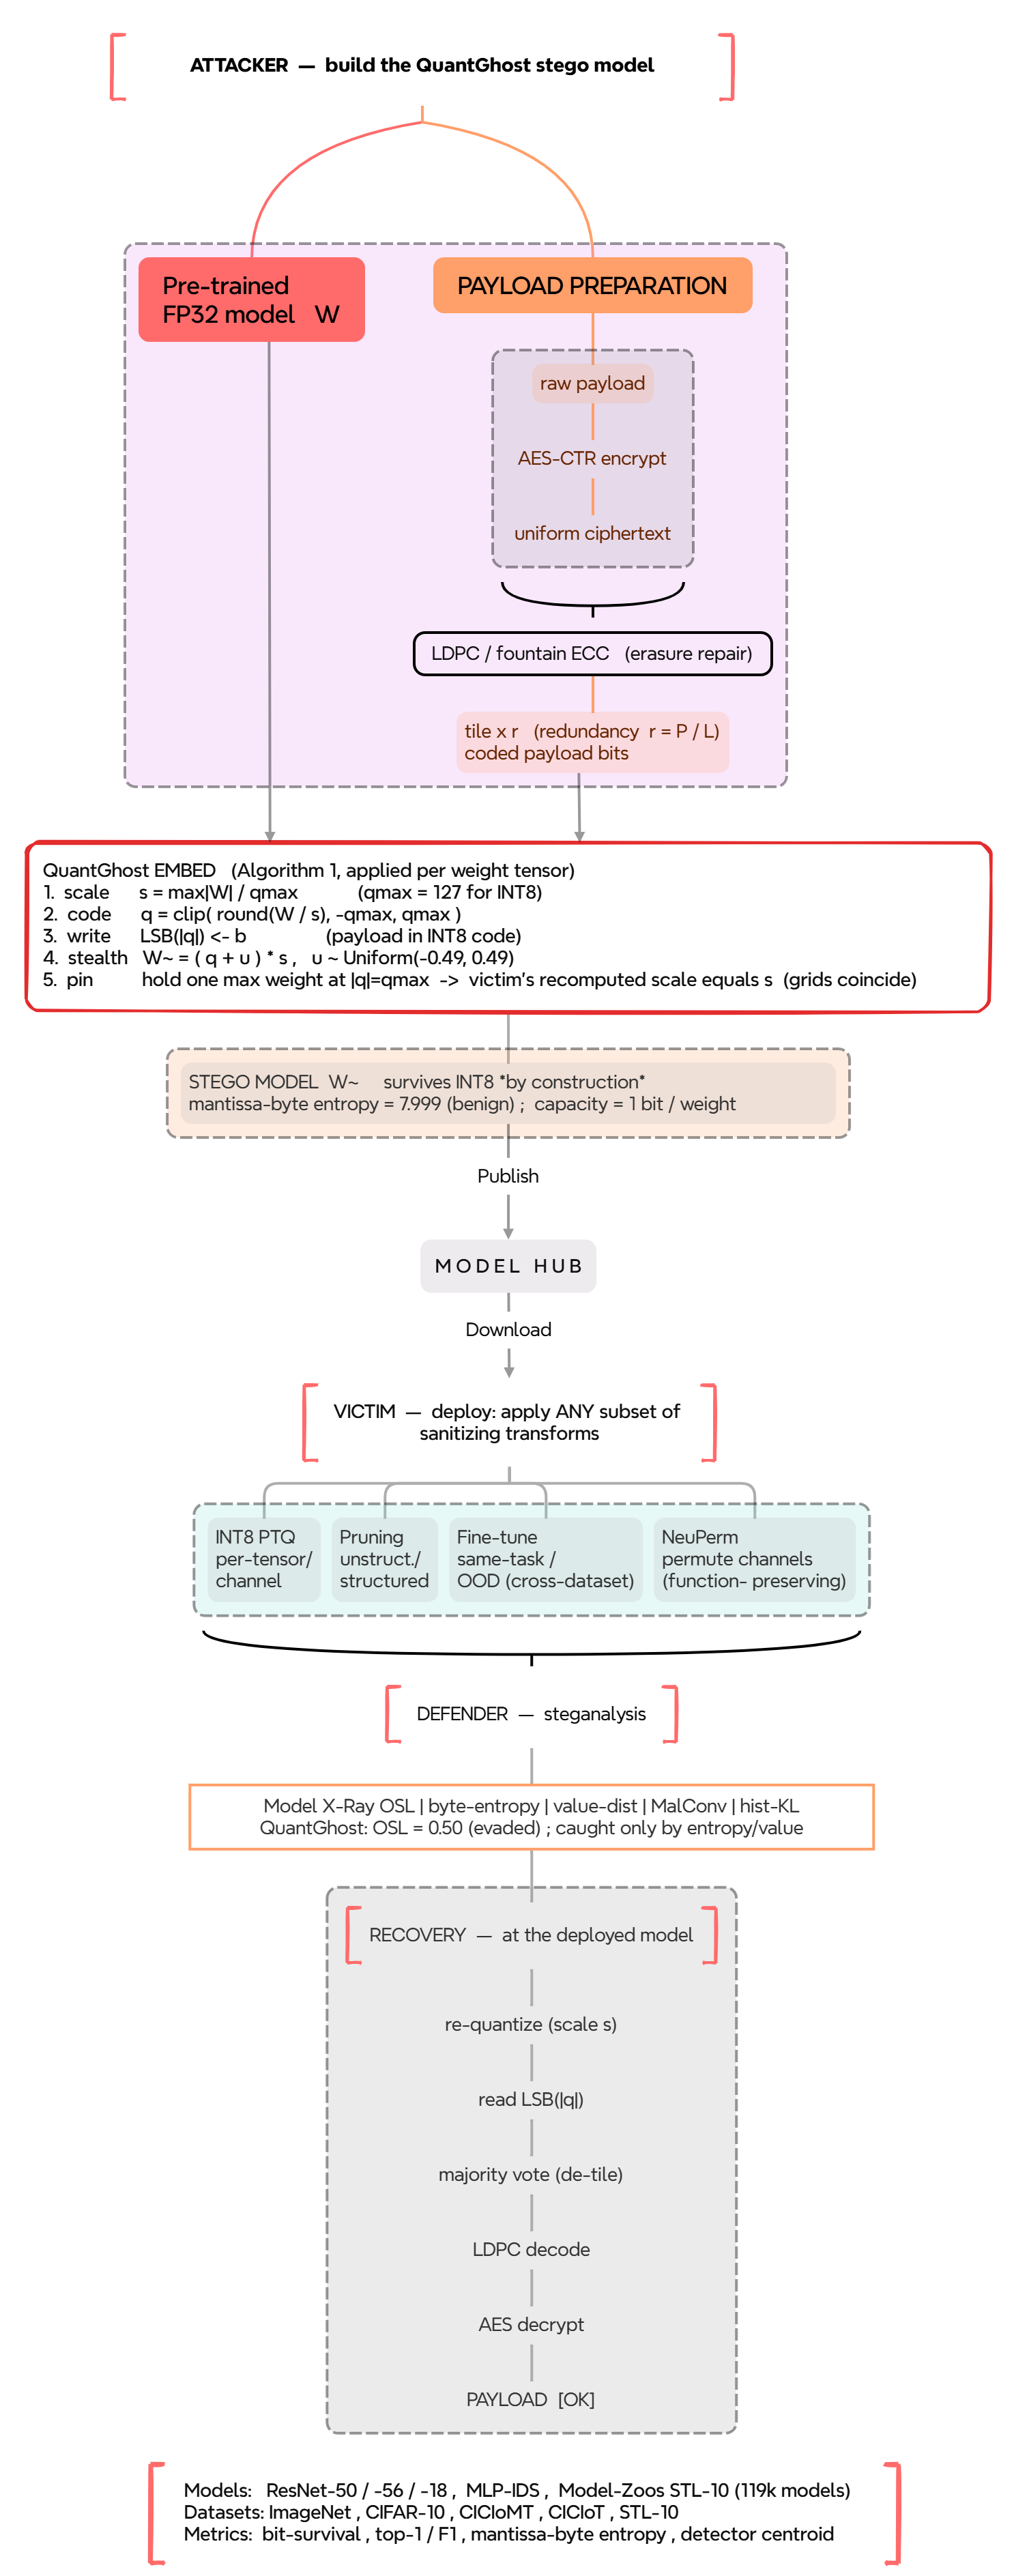
\includegraphics[width=0.50\textwidth]{fig_setupv2.png}
\caption{End-to-end \sys{} pipeline. The attacker embeds an encrypted, error-coded
payload (Algorithm~\ref{alg:embed}) and publishes a benign-looking model; the victim
applies any subset of INT8 quantization, pruning, fine-tuning and NeuPerm; recovery
re-quantizes, reads the code LSBs, and majority-votes.}
\label{fig:setup}
\end{figure}

\subsection{Payload preparation}
Two preprocessing steps make the rest work. First the attacker encrypts the payload
with a stream cipher in counter mode (AES-CTR in our implementation); the ciphertext is
statistically uniform, which is what later lets the embedded bits hide in plain sight.
Second the ciphertext is protected with an erasure code, an LDPC/fountain layer
\citep{luby2002lt}, so that the small number of bit errors that pruning and fine-tuning
inject are repaired exactly at the receiver. The coded stream is then tiled across the
host weights for redundancy, as described in Section~\ref{sec:redund}.

\subsection{Quantization-aware embedding}
The core idea is to stop fighting quantization and instead aim for it. Reading
\eqref{eq:quant} backwards, every float in the half-open bin
\begin{equation}\label{eq:bin}
v\in\big[(q^\star-\tfrac12)s,\ (q^\star+\tfrac12)s\big)
\ \Longrightarrow\ \operatorname{round}(v/s)=q^\star,
\end{equation}
so if we want the victim to read back a code $q^\star$ we are free to choose any value
in that interval. We pick $q^\star$ so that its least significant bit equals the
payload bit, $|q^\star|\bmod 2 = b$. After the victim quantizes, the bit is recovered
by $\hat b=|\!\operatorname{round}(\tilde w/s)|\bmod 2$, exactly, not probabilistically.

One subtlety decides whether this works in practice. The victim recomputes the scale
$s$ from \eqref{eq:quant} on the \emph{modified} weights, and if our edits change the
per-tensor maximum, the grid shifts and recovery drifts. We prevent this by pinning:
the single largest-magnitude weight in each tensor is held at $|q|{=}q_{\max}$ and
carries no payload, so the victim's recomputed scale matches ours and the two grids
coincide. With pinning, survival through quantization is $1.000$ across per-tensor and
per-channel INT8 and even INT4 (Table~\ref{tab:survive}).

\begin{figure}[t]\centering
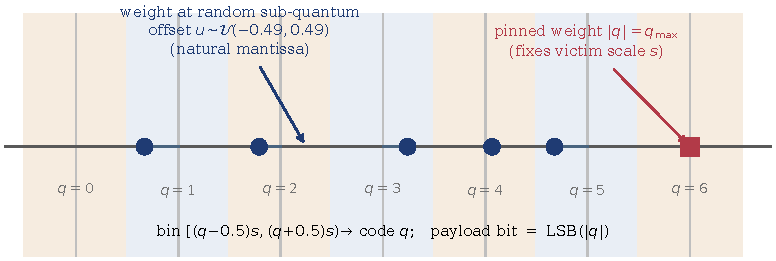
\includegraphics[width=\linewidth]{fig_method.pdf}
\caption{Geometry of the embedding. Each weight is placed at a random sub-quantum
offset inside the INT8 bin whose code $q$ carries the payload bit in its LSB:
re-quantization recovers the bit exactly, while the float mantissa keeps its natural
distribution. One maximum-magnitude weight is pinned to fix the victim's recomputed
per-tensor scale.}
\label{fig:method}
\end{figure}

\subsection{Distribution-preserving stealth}
Snapping weights onto the grid would survive quantization but advertise itself: the
low mantissa byte would take only a handful of values, its entropy would collapse, and
a byte-image detector would separate stego from benign trivially. So we do not snap.
We draw a random offset $u\sim\mathcal{U}(-0.49,0.49)$ and place the weight at
\begin{equation}\label{eq:embed}
\tilde w=\big(q^\star+u\big)\,s,
\end{equation}
which still lands inside the bin \eqref{eq:bin}, survival is untouched, but
leaves the sub-quantum part, the part the mantissa stores, drawn from its natural
in-bin spread. Concretely, writing $\tilde w$ as four bytes and taking the Shannon
entropy of its low mantissa byte,
\begin{equation}\label{eq:entropy}
H=-\sum_{c=0}^{255} p_c\log_2 p_c,\qquad p_c=\Pr[\text{low byte}=c],
\end{equation}
stays at $7.999$ bits, indistinguishable from benign weights, whereas grid-aligned
embedding collapses it. Because the payload was encrypted, the code LSB plane itself is
uniform, so there is no higher-order regularity for a detector to find either.

\begin{algorithm}[t]
\caption{Quantization-aware stealthy embedding (per weight tensor)}
\label{alg:embed}
\begin{algorithmic}[1]
\Require tensor $W$, coded payload bits $\mathbf b$, level $q_{\max}$
\Ensure stego tensor $\tilde W$, scale $s$
\State $s\gets \max_i|W_i|/q_{\max}$;\quad $q\gets\operatorname{clip}(\operatorname{round}(W/s),-q_{\max},q_{\max})$
\State $p\gets\arg\max_i|q_i|$ \Comment{the weight that pins the scale}
\For{each weight index $i$}
  \State $b\gets \mathbf b[\,i \bmod |\mathbf b|\,]$ \Comment{redundant tiling}
  \State $|q_i|\gets(|q_i|\,\&\,{\sim}1)\,\vert\,b$ \Comment{write bit into code LSB}
  \State $u_i\gets\textsc{rand}(-0.49,0.49)$;\ \textbf{if } $i{=}p$ \textbf{ then } $u_i\gets0$
  \State $\tilde W_i\gets\operatorname{sign}(q_i)\,(|q_i|+u_i)\,s$
\EndFor
\State clip $\tilde W$ to $[-q_{\max}s,\,q_{\max}s]$ \Comment{keep victim scale $=s$}
\State \Return $\tilde W,\,s$
\end{algorithmic}
\end{algorithm}

\subsection{Redundancy for pruning and fine-tuning}\label{sec:redund}
Quantization is deterministic, but pruning and fine-tuning move weights around, and a
weight that moves across a bin boundary flips its bit. We absorb this by tiling: bit
$g \bmod L$ is written at weight index $g$, so each of the $L$ message bits is carried
by $r=P/L$ weights ($P$ being the tensor count of embeddable weights). Recovery is a
majority vote,
\begin{equation}\label{eq:vote}
\hat m_j=\mathbf 1\!\Big[\textstyle\sum_{g\,\equiv\, j\,(\mathrm{mod}\,L)} \hat b_g
\ >\ \tfrac12\,\#\{g\equiv j\}\Big],
\end{equation}
which tolerates any corrupted minority. The redundancy $r$ is the dial that trades
capacity for robustness, and it traces the frontier we map in Section~\ref{sec:eval}.

\subsection{A permutation-invariant bootstrap channel}
Neuron permutation is a different kind of threat: it does not change values, it
relabels channels, and a payload indexed by channel position is scrambled wholesale.
The trilemma (Section~\ref{sec:trilemma}) shows this is unavoidable for a high-capacity
positional payload. There is, however, one axis a channel permutation never touches:
the spatial $(k_h,k_w)$ position inside a convolution filter. Embedding a bit that is
replicated across all input and output channels at a fixed spatial tap is therefore
invariant to permutation, and it survives NeuPerm intact. The price is capacity,
$k_h k_w$ bits per conv tensor, but that is exactly enough to deliver the decryption
key or a short URL, which bootstraps the high-capacity channel or an out-of-band fetch.

\subsection{Recovery at the deployed model}
Recovery mirrors the build in reverse and needs only the deployed file. The receiver
recomputes each tensor's scale via \eqref{eq:quant}, reads the code LSBs, de-tiles and
majority-votes \eqref{eq:vote}, runs the erasure decoder to repair the residual errors
(including the pinned weights), and finally decrypts. The only secret that must travel
out of band, or through the invariant channel, is the key.

\subsection{Capacity, complexity, and parameters}\label{sec:analysis}
\paragraph{Capacity.} With $n_{\mathrm{bits}}$ bits per weight, a tensor of $n$ weights
carries $n\,n_{\mathrm{bits}}-\rho$ bits, where $\rho$ is the number of pinned
scale-defining weights ($\rho=1$ for per-tensor and $\rho=C_{\mathrm{out}}$ for
per-channel quantization). The raw aggregate is therefore
$C_{\mathrm{raw}}=n_{\mathrm{bits}}\,P-O(\text{tensors})$, i.e.\ essentially
$P\,n_{\mathrm{bits}}$ bits; at one bit per weight this is $P/8$ bytes
($25.5\,\mathrm{M}\to 3.19$\,MB on ResNet-50). The redundancy and erasure layers trade
this raw figure for reliability, giving a \emph{useful} capacity $C_{\mathrm{raw}}/r$ at
redundancy $r$.

\paragraph{Complexity.} Embedding (Algorithm~\ref{alg:embed}) is a single pass over the
weights: $O(P)$ time and $O(1)$ extra memory beyond the host tensor. Extraction is also
$O(P)$, one re-quantization and LSB read per weight plus an $O(P)$ tally for the majority
vote. Both add negligible overhead to a model load and are independent of the payload
content.

\paragraph{Redundancy and the survival bound.} Let redundancy be $r=P/L$ for an
$L$-bit message, and suppose a transform flips each carrier of a given bit independently
with probability $p<\tfrac12$. The majority vote over $r$ carriers then errs with
probability at most $\exp\!\big(-2r(\tfrac12-p)^2\big)$ by Hoeffding's inequality, so a
target per-bit reliability $\varepsilon$ needs
\begin{equation}\label{eq:redund}
r \;\ge\; \frac{\ln(1/\varepsilon)}{2\,(\tfrac12-p)^2}.
\end{equation}
This is the analytic form of the capacity--robustness frontier we measure empirically:
INT8 quantization gives $p\approx0$ (survival $1.000$ at any $r$, by construction),
$30\%$ pruning gives a small $p$ (survival at modest $r$), and fine-tuning gives a larger
$p$ and hence demands a larger $r$, matching the trends in
Section~\ref{sec:eval}. Structured pruning and out-of-distribution fine-tuning violate
the independence assumption, zeroing or shifting correlated carriers together, which is
why they degrade recovery faster than \eqref{eq:redund} predicts.

\paragraph{Sub-quantum offset.} The offset in \eqref{eq:embed} is drawn from
$\mathcal{U}(-(\tfrac12-\delta),\tfrac12-\delta)$ with a small margin $\delta$ (we use
$\delta=0.01$, i.e.\ $\pm0.49$). The margin keeps every weight strictly inside its bin, so
re-quantization stays exact even under the floating-point rounding that a faithful neuron
permutation introduces; shrinking $\delta\to0$ maximizes mantissa naturalness but risks
boundary crossings, while enlarging it trades a little stealth for a wider safety margin.
The pinned weight uses offset $0$.

% =====================================================================
\section{The capacity-robustness-stealth Trilemma}\label{sec:trilemma}
The bootstrap channel is small for a reason, and the reason is a hard limit rather than
an artefact of our construction. We make it precise (Figure~\ref{fig:trilemma}).

\begin{figure}[t]\centering
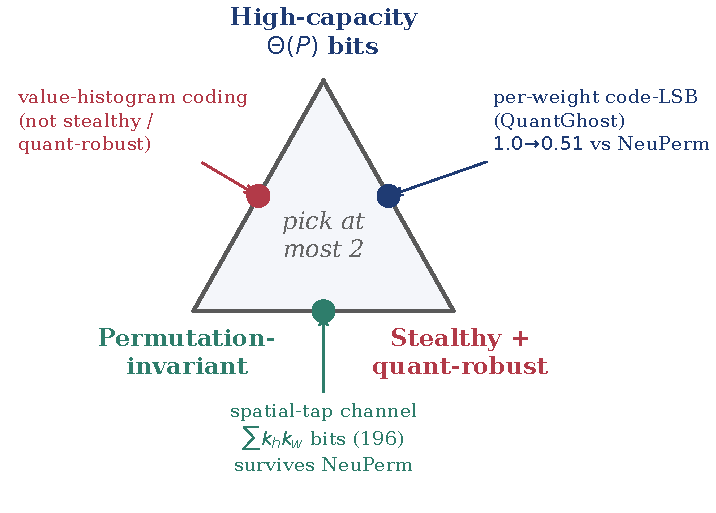
\includegraphics[width=0.85\linewidth]{fig_trilemma.pdf}
\caption{The trilemma. Each embedding occupies one edge, securing the two adjacent
properties and giving up the opposite vertex.}
\label{fig:trilemma}
\end{figure}

\paragraph{Setup.} A convolutional network has weight tensors
$W^{(\ell)}\in\mathbb R^{O_\ell\times I_\ell\times k_h^{(\ell)}\times k_w^{(\ell)}}$
($\ell=1,\dots,L$), with $P=\sum_\ell O_\ell I_\ell k_h^{(\ell)}k_w^{(\ell)}$ weights
and $S_\ell=k_h^{(\ell)}k_w^{(\ell)}$ spatial taps. A function-preserving neuron
permutation is a family $\pi=\{\pi_\ell\in\mathfrak S_{O_\ell}\}$ acting by
$(\pi\!\cdot\!W)^{(\ell)}[o,i,s]=W^{(\ell)}[\pi_\ell^{-1}(o),\pi_{\ell-1}^{-1}(i),s]$,
where the constraint $\sigma_{\ell+1}=\pi_\ell$ keeps residual additions consistent; it
leaves the function unchanged, $f_W=f_{\pi\cdot W}$. Let $G$ be the group of such
permutations. An embedding $(\mathrm{Enc},\mathrm{Dec})$ maps a message $m\in\{0,1\}^C$
and host $W$ to $\tilde W$ with $\mathrm{Dec}(\tilde W)=m$ under a bounded,
accuracy-preserving perturbation.

\begin{definition}[Properties]\label{def:props}
An embedding is \textbf{(P1) high-capacity} if $C=\Theta(P)$; \textbf{(P2)
permutation-invariant} if $\mathrm{Dec}(\pi\!\cdot\!\tilde W)=m$ for all $\pi\in G$; and
\textbf{(P3) stealthy quantization-robust} if $\mathrm{Dec}(Q(\tilde W))=m$ for
per-tensor INT8 $Q$ and the law of $\tilde W$ matches benign weights.
\end{definition}

\begin{lemma}[Position is the only stable identity]\label{lem:pos}
Under \textup{(P3)}, $\mathrm{Dec}$ depends only on the code array $\{q[o,i,s]\}$.
Two weights with the same code are indistinguishable after $Q$, and stealth forbids
using the sub-quantum bits as identity, since fixing them collapses the in-bin law.
Hence a weight's only readable identity is its position $(o,i,s)$.
\end{lemma}

\begin{proposition}[Invariant-capacity bound]\label{prop:bound}
Any embedding satisfying \textup{(P2)} and \textup{(P3)} has
$C\le\sum_{\ell} S_\ell=\sum_\ell k_h^{(\ell)}k_w^{(\ell)}$.
\end{proposition}
\begin{proof}
By Lemma~\ref{lem:pos} the decoder reads a function of the position-indexed codes;
(P2) forces it to be constant on $G$-orbits. $G$ permutes the channel axes $(o,i)$ and
fixes the spatial axis $s$, acting identically across taps. The only positional index
invariant under every $\pi\in G$ is therefore $s\in\{1,\dots,S_\ell\}$. A readout
robust to the value perturbation of $Q$ and to a constant pruning fraction must
aggregate codes sharing an invariant index, i.e.\ a fixed tap, yielding at most one
voted bit per tap per tensor.
\end{proof}

\begin{remark}[Tightness]\label{rem:tight}
The bound is tight. The spatial-tap construction of Section~\ref{sec:method} writes one
bit at each tap, replicated across all $O_\ell I_\ell$ channels, and attains
$C=\sum_\ell S_\ell$ while satisfying (P2) and (P3); the end-to-end recovery of a
$128$-bit key through the full INT8, pruning, and permutation pipeline
(Section~\ref{sec:bootstrap}) realizes it on a real network. Proposition~\ref{prop:bound}
therefore cannot be improved.
\end{remark}

\begin{theorem}[Trilemma]\label{thm:tri}
No embedding satisfies \textup{(P1)}, \textup{(P2)} and \textup{(P3)} at once; each
pair is attainable.
\end{theorem}
\begin{proof}
\emph{(P1)+(P3), not (P2):} the per-weight code-LSB scheme writes one bit per weight,
so $C=\Theta(P)$ and survives $Q$ stealthily, but it is position-indexed
(Lemma~\ref{lem:pos}) and a permutation that moves positions destroys it. \emph{(P2)+(P3),
not (P1):} the spatial-tap scheme meets Proposition~\ref{prop:bound}, $C=o(P)$, and
survives $Q$ and $G$. \emph{(P1)+(P2), not (P3):} the per-tensor value histogram is
$G$-invariant with entropy growing in $P$, but encoding into it reshapes the weight
\emph{value} distribution, breaking (P3) and washed out by $Q$. The first two cases
combined give (P2)$\wedge$(P3)$\Rightarrow C=o(P)$, contradicting (P1).
\end{proof}

\begin{corollary}[The gap is quadratic in width]\label{cor:gap}
The invariant channel is smaller than the positional one by a factor
$P/\sum_\ell S_\ell=\Theta(\overline{O\,I})$. For ResNet-18, $P=1.117\times10^{7}$ while
$\sum_\ell S_\ell=196$, a ratio of about $5.7\times10^{4}$.
\end{corollary}

% =====================================================================
\section{Experimental Setup}\label{sec:setup}
We work with real, pretrained networks rather than toy proxies: ResNet-50
\citep{he2016resnet} on ImageNet \citep{deng2009imagenet} for capacity, ResNet-56 on
CIFAR-10 \citep{krizhevsky2009cifar} for accuracy, pruning and fine-tuning, and
ResNet-18 on ImageNet for neuron permutation and the prior-art baselines. Quantization
follows the standard per-tensor symmetric INT8 (and INT4) scheme of \eqref{eq:quant}
\citep{nagel2021whitepaper}.
For steganalysis we run the released Model X-Ray OSL detector
\citep{gilkarov2026modelxray}, the Grayscale-Fourpart representation with a
metric-learning few-shot head, scored by centroid and $1$-NN, together with a panel
of byte-level detectors: a MalConv-style 1D-CNN, a low-byte entropy test, a
value-distribution test, a histogram-KL test, and a byte-autocorrelation test. The
benign population is the diverse Model Zoos STL-10 small-CNN collection
\citep{schurholt2022modelzoos} of roughly $1.2\times10^{5}$ models; few-shot support is
$20{+}20$ over five repeats. Payloads are encrypted random
bytes for the stealth and capacity studies, and real benign binaries for the
structured-payload regime in which the naive attack is actually detectable. We report
bit-survival and bit-recovery (chance $0.5$), top-1 accuracy or F1, mantissa-byte
entropy \eqref{eq:entropy}, and detector centroid/AUC.

% =====================================================================
\section{Evaluation}\label{sec:eval}
\subsection{Survival through quantization}
Table~\ref{tab:survive} confirms the by-construction claim. The naive payload is erased
($0.50$); ours survives at $1.000$ for per-tensor and per-channel INT8 and for INT4,
with mantissa entropy pinned at the benign $7.999$. INT4's coarser bins cost accuracy
but not survival, which is consistent with the geometry of \eqref{eq:bin}.

\begin{table}[t]\centering
\caption{Survival through quantization on real models (chance $0.5$).}
\label{tab:survive}
\begin{tabular*}{\columnwidth}{@{\extracolsep{\fill}}lccc@{}}
\toprule
Scheme & survival & embed acc. & mant. entropy\\
\midrule
naive X-LSB (INT8) & 0.500 & n/a & n/a\\
ours, per-tensor INT8 & \textbf{1.000} & 0.475 & 7.999\\
ours, per-channel INT8 & \textbf{1.000} & 0.488 & 7.999\\
ours, per-tensor INT4 & \textbf{1.000} & 0.138 & 7.999\\
ours, per-channel INT4 & \textbf{1.000} & 0.196 & 7.998\\
\bottomrule
\end{tabular*}
\end{table}

\subsection{Accuracy is preserved}
On a real CIFAR-10 ResNet-56 (top-1 $94.25\%$) the full attack barely moves the needle
(Table~\ref{tab:acc}). Embedding a $106$\,KB payload and then applying the victim's
INT8 quantization costs $0.19$ percentage points, and the payload comes back at
$99.997\%$ before error correction. Quantization alone accounts for almost none of the
loss, which tells us the residual is the embedding's own sub-quantum nudge.

\begin{table}[t]\centering
\caption{Accuracy preservation on a real CIFAR-10 ResNet-56. $106$\,KB payload, recovery $99.997\%$.}
\label{tab:acc}
\begin{tabular*}{\columnwidth}{@{\extracolsep{\fill}}lc@{}}
\toprule
Condition & top-1\\
\midrule
original FP32 & 94.25\%\\
clean INT8 & 94.24\%\\
embed FP32 & 93.97\%\\
embed $+$ INT8 (victim) & 94.06\%\\
\midrule
$\Delta$ (orig $\to$ embed$+$INT8) & $-0.19$\,pp\\
\bottomrule
\end{tabular*}
\end{table}

\subsection{Capacity and comparison with prior art}
On ResNet-50 ($25.5$M weight parameters) a $3.19$\,MB encrypted payload survives
FP32$\to$INT8 at $99.9999\%$, and the handful of residual errors, one pinned weight
per tensor, are repaired by the erasure layer for byte-exact delivery.
Table~\ref{tab:baseline} sets this against prior art on a real ResNet-18: the naive
attack is erased at every depth, while ours survives. Robust watermarking
\citep{tondi2022robust,li2021stdm} occupies the opposite corner, robust and stealthy
but capped at a couple of kilobytes, which is the trade we explain in
Section~\ref{sec:trilemma}.

\begin{table}[t]\centering
\caption{Baselines under INT8 on a real ResNet-18 (chance $0.5$).}
\label{tab:baseline}
\begin{tabular*}{\columnwidth}{@{\extracolsep{\fill}}lcc@{}}
\toprule
Method & capacity & survival INT8\\
\midrule
EvilModel/StegoNet $X{=}8$ & 8\,bit/w & 0.500 (erased)\\
EvilModel/StegoNet $X{=}16$ & 16\,bit/w & 0.500 (erased)\\
EvilModel/StegoNet $X{=}23$ & 23\,bit/w & 0.501 (erased)\\
robust watermark & $\le$2\,KB & robust (low-cap)\\
\textbf{\sys} & 1\,bit/w & \textbf{1.000}\\
\bottomrule
\end{tabular*}
\end{table}

\subsection{Stealth against detectors}
Stealth is not uniform across detectors, and we report the full result (Figure~\ref{fig:detectors},
Table~\ref{tab:stealth}). Against the released Model X-Ray detector our embedding sits
at chance ($0.50$) on a diverse model population, while the naive attack is detected
($0.81$); the detector plainly works, it simply cannot separate ours from benign. We
initially measured a higher number ($0.75$) on a small, homogeneous pilot zoo, but that
turned out to be an artefact, near-identical benign models inflate few-shot
separability, and it vanishes once the population is realistically diverse. Across
the byte-level panel ours evades MalConv, histogram-KL and byte-autocorrelation
(all near $0.5$) and is caught only by the entropy and value-distribution tests, which
pins down precisely which two detectors a defender should keep.

\begin{figure}[t]\centering
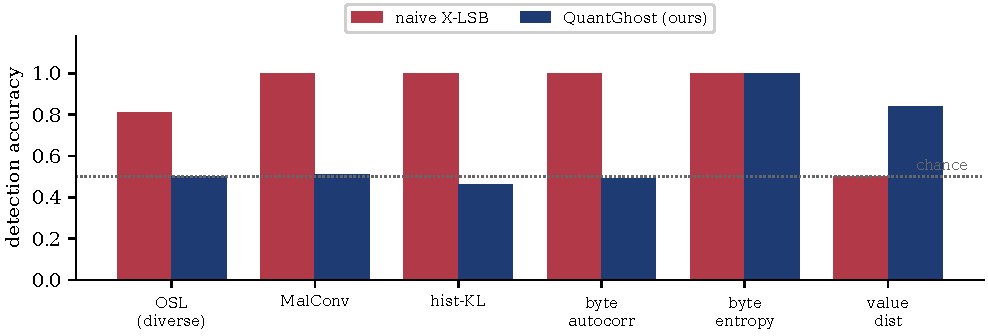
\includegraphics[width=\linewidth]{fig_detectors.pdf}
\caption{Detection accuracy (chance $0.5$) of the naive attack and ours across six
detectors. Ours evades four; only byte-entropy and value-distribution catch it.}
\label{fig:detectors}
\end{figure}

\begin{table}[t]\centering
\caption{Stealth against the released Model X-Ray OSL detector. Diverse zoo, $20{+}20$
support, five repeats.}
\label{tab:stealth}
\begin{tabular*}{\columnwidth}{@{\extracolsep{\fill}}lccc@{}}
\toprule
Population & attack & centroid & 1-NN\\
\midrule
homogeneous (artefact) & ours & 0.747 & 0.681\\
diverse & naive X-LSB & 0.807 & 0.794\\
diverse & \textbf{\sys} & \textbf{0.504} & \textbf{0.508}\\
\bottomrule
\end{tabular*}
\end{table}

\subsection{Pruning and fine-tuning}
Survival under pruning is reported in Figure~\ref{fig:prune} and Table~\ref{tab:prune}.
The pattern is clean: there is no operating point that removes the payload and keeps the
model. Unstructured pruning leaves the payload fully recoverable at $30\%$ (accuracy
$93.8\%$) and only erases it at $70$--$90\%$, where accuracy has itself fallen to
$78\%$ and then $20\%$. Structured pruning destroys the model at every ratio, the
accuracy is already at chance, while the payload partly survives, so it is not a
useful sanitizer either. Fine-tuning is gentler still: three epochs of same-task
training leave recovery at $1.000$ for both high and modest redundancy
($3326\times$ and $207\times$) with accuracy at $94.2\%$. Only a harsher, out-of-distribution
fine-tune bites, as we show next.

\begin{figure}[t]\centering
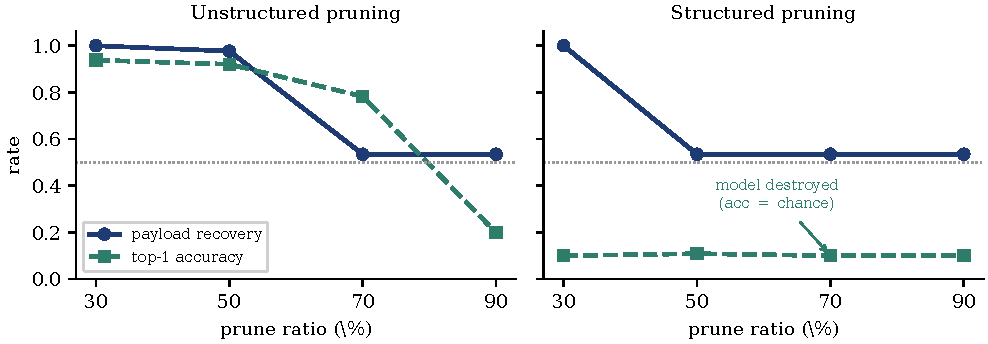
\includegraphics[width=\linewidth]{fig_prune.pdf}
\caption{Pruning on a real ResNet-56: payload recovery and top-1 accuracy versus
ratio. The payload only dies where accuracy also dies; structured pruning destroys
the model at every ratio.}
\label{fig:prune}
\end{figure}

\begin{table}[t]\centering
\caption{Pruning on real ResNet-56 (recovery / top-1), redundancy $3326\times$.}
\label{tab:prune}
\begin{tabular*}{\columnwidth}{@{\extracolsep{\fill}}lcc@{}}
\toprule
Prune ratio & unstructured & structured\\
\midrule
30\% & 1.000 / 93.8\% & 1.000 / 10.0\%\\
50\% & 0.977 / 92.1\% & 0.535 / 10.9\%\\
70\% & 0.535 / 78.3\% & 0.535 / 10.0\%\\
90\% & 0.535 / 19.9\% & 0.535 / 10.0\%\\
\bottomrule
\end{tabular*}
\end{table}

\subsection{Neuron permutation at real scale}
Table~\ref{tab:neuperm} reports a faithful neuron permutation on a real ResNet-18,
implemented with the residual, batch-norm and downsample bookkeeping that a correct
permutation requires. We verified it is function-preserving to machine precision: the
logit difference is $1.1\times10^{-14}$ in float64, so accuracy is identical by
construction and needs no measurement. The high-capacity positional payload is
destroyed ($1.000\!\to\!0.508$), exactly as the trilemma predicts, but the spatial-tap
channel survives untouched ($1.000\!\to\!1.000$) at $196$ bits across the network's $20$
conv tensors. NeuPerm thus pins the attacker to the low-capacity corner without closing
the channel.

\begin{table}[t]\centering
\caption{Faithful NeuPerm on real ResNet-18 ($11.2$M conv weights, $\Delta_{\mathrm{fp64}}=1.1\times10^{-14}$).}
\label{tab:neuperm}
\begin{tabular*}{\columnwidth}{@{\extracolsep{\fill}}lcc@{}}
\toprule
Channel & no perm & after NeuPerm\\
\midrule
positional (high-capacity) & 1.000 & 0.508 (chance)\\
spatial-tap (invariant, 196\,bit) & 1.000 & \textbf{1.000}\\
\bottomrule
\end{tabular*}
\end{table}

\subsection{End-to-end bootstrap: defeating NeuPerm}\label{sec:bootstrap}
Although the surviving channel is small, it is operationally sufficient, as we
demonstrate end to end on a real ResNet-18. The
attacker encrypts a $4$\,KB payload with a random AES-128 key, places the ciphertext in
the high-capacity positional channel, and places the $128$-bit key in the
permutation-invariant spatial channel (capacity $196$ bits, so the key fits with room to
spare). The victim then applies the entire pipeline at once: per-tensor INT8
quantization, $30\%$ unstructured pruning, and a faithful neuron permutation. After this
chain, the positional payload in the weights is gone (recovery $0.50$, chance), exactly
as the trilemma predicts. The key, however, is recovered \emph{bit-exactly}
($128/128$), and using it to decrypt the ciphertext, which the attacker delivers out of
band, returns the original $4$\,KB payload \emph{byte-for-byte}. The strongest single
defense in the literature therefore bounds the attacker to the low-capacity corner but
does not close the channel: a few hundred surviving bits are enough to carry a key that
bootstraps the full payload. This is the operational meaning of an ``incomplete''
sanitizer, and it is why Section~\ref{sec:defenses} argues that permutation must be
paired with explicit inspection of the invariant spatial statistics.

\subsection{Cross-architecture and cross-dataset ablation}\label{sec:ablation}
Because the embedding manipulates raw weights, nothing about it is specific to vision
or to convolutions. Table~\ref{tab:ablation} bears this out on a tabular
network-intrusion MLP trained on CICIoMT \citep{dadkhah2024ciciomt2024} for binary
benign-versus-attack detection (F1 $0.989$). The $1664$\,B payload survives INT8 at
$1.000$ and accuracy and F1 are unchanged across all four conditions. Two things are
worth drawing out. The MLP has only three linear tensors and no spatial taps, so its
permutation-invariant capacity is just three bits against $196$ for ResNet-18, the
bound of Proposition~\ref{prop:bound} holding across architectures, since a dense layer
is the $k_h k_w=1$ case. And a genuinely cross-dataset fine-tune, taking the model from
CICIoMT to CICIoT \citep{neto2023ciciot2023} over the shared feature space, adapts the
detector (F1 $0.930\!\to\!0.982$) and, unlike same-task fine-tuning, breaks the payload
at $208\times$ redundancy ($0.469$, chance). The lesson is that it is transform
severity, not transform type, that sets the surviving capacity.

\begin{table}[t]\centering
\caption{Cross-architecture / cross-dataset ablation on a tabular IDS MLP.}
\label{tab:ablation}
\begin{tabular*}{\columnwidth}{@{\extracolsep{\fill}}lc@{}}
\toprule
Quantity & value\\
\midrule
IDS F1 (orig $\to$ embed$+$INT8) & $0.989\to0.989$\\
accuracy (orig $\to$ embed$+$INT8) & $97.85\%\to97.85\%$\\
payload survival INT8 (MLP) & \textbf{1.000}\\
invariant capacity (FC vs conv) & 3 bits vs 196\\
cross-dataset fine-tune (F1) & $0.930\to0.982$\\
\quad payload after that fine-tune & 0.469 (chance, $208\times$)\\
\bottomrule
\end{tabular*}
\end{table}

% =====================================================================
\section{A Targeted Detector for \sys}\label{sec:detector}
The byte-level and gf-image steganalyzers of Section~\ref{sec:eval} fail against \sys{}
because they look in the wrong place: the mantissa-byte distribution is preserved
(entropy $7.999$) and the float value distribution is benign on a diverse population.
The exploitable signal is one level down, in the \emph{sub-quantum residual}. By
construction \sys{} places each weight at a uniform offset inside its bin, so the
residual $r=w/s-\mathrm{round}(w/s)$ is (near-)uniform; a benign tensor's residual instead
carries a model-specific, non-uniform shape, since most trained weights are small and
concentrate the residual. We turn this into a concrete detector.

\paragraph{Detector.} For each weight tensor we histogram the residual into $B{=}40$ bins
over $[-\tfrac12,\tfrac12)$; the per-model feature is the mean histogram across tensors,
and a logistic-regression classifier separates benign from stego. The detector is
cheap, one pass over the weights, and uses no labels of the payload itself.

\paragraph{Result.} On the CIFAR carrier zoo with five-fold cross-validation
(Table~\ref{tab:detector}) the residual detector reaches ROC-AUC $1.000$ against the
basic \sys{} embedding, where the mantissa-entropy baseline that prior steganalysis
relies on is exactly at chance ($0.500$). The targeted detector therefore closes the
stealth gap that the byte-level detectors leave open.

\paragraph{Adaptive attacker.} A natural counter is to widen the offset to the full bin
and drop the exact-zero pin signature. This adaptive \sys{} lowers the detector to
AUC $0.771$, still well above chance: the scale-defining weight must remain pinned for the
payload to survive quantization, and a perfectly uniform residual is itself anomalous
against the benign shape. To fall back to chance the attacker would have to sample
offsets from the \emph{benign} residual law, which forfeits the freedom the channel
relies on and lowers usable capacity. The residual test thus raises the cost of stealth
sharply, and it composes with the structural defense of Section~\ref{sec:defenses}: an
attacker who matches the residual is still bounded by neuron permutation to the
low-capacity invariant channel.

\begin{table}[t]\centering
\caption{Proposed sub-quantum residual detector versus the mantissa-entropy baseline,
five-fold cross-validated ROC-AUC on the CIFAR carrier zoo (chance $0.5$).}
\label{tab:detector}
\begin{tabular*}{\columnwidth}{@{\extracolsep{\fill}}lc@{}}
\toprule
Detector vs.\ attacker & ROC-AUC\\
\midrule
mantissa entropy vs.\ basic \sys{} & 0.500\\
residual histogram vs.\ basic \sys{} & \textbf{1.000}\\
residual histogram vs.\ adaptive \sys{} & 0.771\\
\bottomrule
\end{tabular*}
\end{table}

% =====================================================================
\section{Defenses}\label{sec:defenses}
Reading the results as a defender, no single mechanism is enough, but a small
combination is. We take each lever in turn.

\paragraph{Transforms are not clean sanitizers.} Quantization sanitizes the prior art
and nothing else. Pruning, on a real model, never separates the payload's death from
the model's: the bits go only when accuracy has already gone (Table~\ref{tab:prune}),
and structured pruning simply breaks the network. Light fine-tuning leaves the payload
in place; only an out-of-distribution fine-tune, which a benign deployer may not have a
reason to run, bounds it.

\paragraph{Two detectors that work, and an arms race.} Among the detectors we tried,
the entropy and value-distribution tests are the ones that catch our embedding
(Figure~\ref{fig:detectors}); the gf-image OSL detector and the rest do not, once the
benign population is diverse. But even those two invite an arms race. Because they read
the marginal value distribution, switching from a single global scale to a per-tensor
scale lowers their accuracy from $0.98$ to $0.84$, better stealth against them, and,
just as the trilemma says, no help against the structural detector. The take-away for
detection is to stop looking for distributional anomalies in the floats, which a careful
attacker removes, and to look one level down at the sub-quantum residual: the targeted
detector of Section~\ref{sec:detector} catches \sys{} at AUC $1.000$ and still scores
$0.771$ against an adaptive attacker, which is the most reliable signal we found.

\paragraph{NeuPerm and the residual.} NeuPerm is the strongest single defense and it
does its job on the high-capacity channel (Table~\ref{tab:neuperm}). What it cannot do,
by Theorem~\ref{thm:tri}, is remove the $\sum_\ell k_h k_w$-bit invariant channel,
which is ample for a key or a URL.

\paragraph{What a complete sanitizer needs.} Putting these together, a defender who
wants to actually close the channel must (i) bound the positional capacity with heavy
quantization or stochastic weight perturbation, (ii) apply neuron permutation to remove
it, and (iii) inspect the permutation-invariant spatial statistics the residual channel
is forced to use, alongside the entropy and value-distribution detectors and a code
low-bit predictability test. Each piece is partial; only their conjunction covers all
three corners of the trilemma. The open costs are the operational price of routinely
permuting shipped models, it rewrites the artefact and can break tooling that
assumes a canonical channel order, and the false-positive rate of predictability
testing on benign models.

% =====================================================================
\section{Discussion and Limitations}\label{sec:disc}
We state the main limitations explicitly. Our accuracy and pruning studies use
CIFAR-scale and IDS-scale models where a full transform sweep is affordable; the
capacity result is on ImageNet-scale ResNet-50 but without a top-1 number, which would
require the ImageNet validation set we did not assume access to. The neuron-permutation
analysis covers the BasicBlock ResNet family in full and a fully-connected IDS model;
extending the faithful permutation to transformer blocks is mechanical but not done
here. Our proposed residual detector (Section~\ref{sec:detector}) is evaluated on the
CIFAR carrier zoo; testing it across larger and more diverse benign populations, and
co-evolving the adaptive attacker and the detector to a fixed point rather than one round,
are the natural next steps. Finally, the trilemma is stated for the channel-permutation
group of convolutional and dense layers; richer symmetry groups (for example scaling
symmetries across ReLU boundaries) would only tighten, not loosen, the invariant-capacity
bound.

% =====================================================================
\section{Ethics and Responsible Disclosure}\label{sec:ethics}
This is offensive research carried out to strengthen defenses. Every payload in our
experiments is either encrypted random bytes or a benign binary; at no point is live
malware embedded, executed, or distributed. The threat we describe is against published
detectors and defenses, and we will disclose our findings to the authors of Model X-Ray
and NeuPerm ahead of publication, together with the mitigations of
Section~\ref{sec:defenses}. We release our code to support reproducibility and
defensive follow-up.

% =====================================================================
\section{Conclusion}\label{sec:concl}
\sys{} shows that payloads hidden in neural-network weights can be made to ride through
the entire deployment pipeline, INT8 quantization, pruning, and fine-tuning, while
keeping accuracy (down $0.19$ points on a real ResNet-56) and slipping past the released
Model X-Ray detector on a realistic model population, demonstrated at $3.2$\,MB on a real
ResNet-50. Behind the construction sits a clean impossibility: capacity, robustness and
stealth cannot all be had at once, and the permutation-invariant channel is bounded by
$\sum_\ell k_h k_w$ bits. On a real ResNet-18 a faithful neuron permutation erases the
big payload but leaves that $196$-bit channel standing, which is enough to bootstrap
recovery. Deployment transforms, NeuPerm among them, do not by themselves sanitize a
shared model; doing so takes permutation \emph{plus} inspection of the very statistics
the surviving channel is forced to expose. We hope the trilemma and the detectors it
points to give defenders a concrete target.

% =====================================================================
\section*{Acknowledgements}
The authors gratefully acknowledge the Media and Games Innovation Centre of Excellence
(MaGIC-X), Universiti Teknologi Malaysia, for supporting this research through its
technical resources and computing facilities. This work was funded by Universitas
Dinamika Bangsa, Jambi, Indonesia.

% =====================================================================
\section*{CRediT authorship contribution statement}
\textbf{Eko Arip Winanto:} Conceptualization, Methodology, Software, Formal analysis,
Investigation, Writing -- original draft. \textbf{Mohd Yazid Idris:} Supervision,
Conceptualization, Funding acquisition, Writing -- review \& editing.
\textbf{Kurniabudi:} Validation, Data curation, Writing -- review \& editing.

\section*{Declaration of competing interest}
The authors declare that they have no known competing financial interests or personal
relationships that could have appeared to influence the work reported in this paper.

\section*{Data and code availability}
The datasets used are publicly available: CIFAR-10, ImageNet, the STL-10 Model Zoos
collection \citep{schurholt2022modelzoos}, CICIoT2023 \citep{neto2023ciciot2023}, and
CICIoMT2024 \citep{dadkhah2024ciciomt2024}. The source code and scripts that reproduce
all experiments, tables, and figures will be released in a public repository upon
acceptance, and are available from the corresponding author on reasonable request in
the meantime. No live malware is included in the release.

\section*{Ethical and responsible-disclosure note}
All payloads in this study are encrypted random bytes or benign binaries; no live
malware is embedded, executed, or distributed. The authors will disclose the findings to
the authors of the affected detector and defense (Model X-Ray and NeuPerm) prior to
publication.

\bibliographystyle{cas-model2-names}
\bibliography{references}

\end{document}
